% ESG -- environmental sustainability G ???

% Checklist and TO DOs
% Describe metodology of the work with sources
% Classification of Benchmarks
% add Pros and Cons of my approach compared with anothers
% why do most benchmark use fixed sets of tasks
% why do we need a modular benchmark
% What do benchmarks check
  % Categories of tasks: Math, Logic, Table understanding,  Reading comprehension, Commonsense reasoning, Vision \cite{vendrow2025largelanguagemodelbenchmarks}
%
% Why did I chose Java and Spring Boot instead of Python (because Spring AI is great), and React
% Mention that I used OpenRouter, but any provided supported by Spring AI could be used
%
% Focus more on the concept of benchmarks with UI, than in the implementation

\section{Introduction}

Large Language Models (LLMs) have significantly impacted software development through AI-assisted programming tools like GitHub Copilot and Cursor.
However, evaluating and fine-tuning these models requires extensive benchmarking~(\cite{paul2024benchmarksmetricsevaluationscode}), which comes with significant computational, financial, and environmental costs.
Current benchmarks often include irrelevant tasks (\cite{vendrow2025largelanguagemodelbenchmarks}) and offer limited customization, making them inefficient for specific use cases~(\cite{yang2023intercodestandardizingbenchmarkinginteractive}).

This work explores existing benchmarks for code-generating LLMs and proposes a novel approach: an easily customizable benchmark with detailed, easily analyzable outputs that can be tailored to specific needs while remaining cost-effective and environmentally conscious.

This master thesis began with a comprehensive literature review, using recent critical reviews as a foundation for analyzing the state of LLM benchmarking.
The review was extended by following citations to relevant articles published in late 2024 and 2025, focusing on keywords related to benchmarking and LLMs.
The findings from this literature analysis informed the design and implementation of a modular benchmarking system, which was then evaluated for efficiency, flexibility, and environmental impact.

The literature review and further research were guided by the following questions:
\begin{itemize}
    \item RQ1: What are the main limitations of current LLM benchmarks for code generation?
    \item RQ2: What metrics best reflect real-world usability and code quality?
    \item RQ3: How can benchmarks be made customizable for different user needs?
    \item RQ4: What is the environmental impact of repeated benchmarking, and how can it be reduced?
\end{itemize}

\textbf{Main contributions of this work:}
% GLuque: En la versión final evita estos saltos de líneas entre este "título" y el texto siguiente. Quizás una forma simple es con \newpage, pero esto es para la versión final ya que si cambias cosas puede afectar y que esté bien.
\begin{itemize}
    \item A critical analysis of existing LLM code generation benchmarks and their shortcomings.
    \item The design and implementation of a modular, customizable benchmarking framework.
    \item Consideration of environmental and cost factors in the benchmarking process.
    \item An interactive web interface for configuring benchmarks and analyzing results.
\end{itemize}

\subsection{Problem Statement}

Benchmarking LLMs for code generation is essential for both research and practice, but current approaches face critical limitations.
Most benchmarks are fixed datasets, which leads to task saturation and data leakage as models are trained on their contents~(\cite{paul2024benchmarksmetricsevaluationscode}).
The lack of customization prevents researchers and practitioners from focusing on tasks relevant to their use cases/ % (\cite{}) ?
At the same time, running large benchmarks consumes significant computational resources, resulting in high costs and environmental impact.
Furthermore, benchmark outputs are often limited to single numeric metrics, which fail to capture nuanced aspects of model performance such as efficiency, style, or error patterns.

Therefore, this thesis addresses the lack of a flexible, customizable, and sustainable benchmarking framework for evolving LLM capabilities and user needs.

\subsection{Objectives}

The main objectives of this work are:
\begin{enumerate}
    \item Conduct a detailed analysis of existing benchmarks and identify their limitations.
    \item Design a modular benchmarking system that enables:
    \begin{itemize}
        \item Custom task selection and filtering.
        \item Configuration of evaluation criteria.
        \item Support for multiple programming languages and task types.
        \item Integration with CI/CD pipelines for automated benchmarking.
    \end{itemize}
    \item Implement an interactive web interface for benchmark configuration and result analysis.
    \item Develop a cost-efficient and environmentally conscious approach to benchmarking.
\end{enumerate}

The goal of this work is not to compete with large-scale frameworks, but to present a prototype that illustrates a different approach: a benchmarking tool for LLMs with a graphical user interface and configuration-driven design.
Instead of hard-coded pipelines, users can flexibly define tasks, parameters, and evaluation criteria through configuration files generated using the UI.

\subsection{Relevance of the Work}

The relevance of this work lies in addressing the growing inefficiency and environmental cost of LLM benchmarks.
By introducing a customizable framework, this thesis provides a practical solution for researchers and practitioners who need targeted, resource-efficient evaluations.
The proposed system not only reduces time and energy consumption but also enhances the practical relevance of benchmarking results.

\subsection{Organization of this document}

This document is composed of 5 chapters and 3 appendices.
The content of each one is:
\begin{enumerate}
    \item In the Chapter ``State of Art'', we analyze the existing benchmarks, and how they solved the problems of the ones before them.
    Then we examine in detail the shortcomings and limitations of the existing benchmarks.
    In the same chapter, we also explore the existing LLM benchmarking frameworks.
    Based on the performed analysis of the State of the Art, we respond our Research Questions.
    \item In the following chapter ``Design of the Modular Benchmarking Framework'', we introduce a new approach to benchmarking LLMs, describing the overall idea and its expected benefits.
    \item In the Chapter ``Implementation of the Modular Benchmarking Framework'', we dive into an implementation of a prototype based on the concept, described in the previous chapter.
    First, we describe the way to interact with the benchmark, the file structure, and then demonstrate the frontend application.
    \item In the Chapter ``Results and Evaluation'' we conduct the experimental runs, analyze their results, and compare the prototype with the existing benchmark frameworks.
    \item Finally, in the Chapter ``Conclusion and Future Work'', we describe the work that was done, and if the proposed idea is viable.
    We finish by defining the future work related to the presented concept.
    \item The Appendices contain a Sequence Diagram describing user interaction with the proposed framework, a number of screenshots of a UI, and finally the examples of the files that the framework manages.
\end{enumerate}

\section{State of the Art}

In this chapter, we analyze the existing benchmarks, and how they evolved and were developed to overcome the limitations of their predecessors.
After this analysis, we highlight the main limitations and shortcomings of the existing benchmarks.
Then, we explore the existing LLM benchmarking frameworks and their limitations.
Finally, we respond to our Research Questions based on the performed analysis of the State of the Art.

\subsection{Evolution of Code Generation Benchmarks}

The evolution of benchmarks for code generation has been driven by the need to evaluate the capabilities of Large Language Models (LLMs) in programming tasks.
Early benchmarks focused on isolated tasks, but as LLMs became more sophisticated, the need for more comprehensive and realistic evaluation methods emerged~(\cite{paul2024benchmarksmetricsevaluationscode}).

The first benchmarks were aimed at text comprehension and contained questions and expected answers, such as GLUE, SQuAD, and GSM8K with grade-school math problems~(\cite{vendrow2025largelanguagemodelbenchmarks}).

As LLM capabilities expanded, benchmarks shifted towards programming tasks, with a focus on code generation and understanding.
Some pioneers in LLM code benchmarking are MBPP, HumanEval, and APPS.

\begin{itemize}
\item MBPP (Mostly Basic Python Problems), published by~\cite{austin2021program}, contains $974$ crowdsourced Python programming problems with tests.

\item HumanEval was developed at OpenAI by~\cite{chen2021evaluatinglargelanguagemodels} with $164$ hand-crafted problems, aiming to avoid data leakage (ensuring that the problems and golden solutions are not present in the training dataset).

\item APPS by~\cite{hendrycksapps2021} features $10,000$ Python tasks with $131,777$ test cases, borrowed from open-access sites like Codewars and Codeforces.
\end{itemize}
These benchmarks are still used today for comparing the performance of different models in scientific papers.
Notably, APPS benchmark is commonly used for fine-tuning LLMs for programming tasks, as it allows the use of separate sets of problems for training and evaluation~(\cite{bigcode-evaluation-harness}).

The mentioned benchmarks became less effective as newer models were trained on the same tasks they are being evaluated on.
This phenomenon is known as \textbf{data leakage}, as described by~\cite{vendrow2025largelanguagemodelbenchmarks}.

Amazon's Recode benchmark~\cite{recode_wang2022} addressed this issue by introducing perturbations on docstrings, function names, and code, while staying semantically close to the original task.
However, this is more a way to test the robustness of the model rather than its ability to solve brand-new problems.

More recent developments like HumanEval Pro and MBPP Pro~\cite{yu2024humanevalprombpppro} introduced more sophisticated testing approaches.
Their multistep evaluation process tests an LLM's ability to work with its own generated code.
First, an LLM generates a solution to a known problem from HumanEval or MBPP datasets.
Then, it is given a new task that requires calling a function generated in the first step.
This approach revealed limitations in some models that perform well on simpler tasks.

The mentioned academic benchmarks focus on controlled and isolated tasks, while SWE-bench (\cite{jimenez2024swebenchlanguagemodelsresolve}) moved toward real-world scenarios.
Software engineering tasks were taken from resolved issues from GitHub repositories of open-source Python projects.
SWE-bench is famous for its leaderboards, where laboratories and companies worldwide compete to achieve the highest percentage of solved tasks.
However, the benchmark is limited to tasks from only 12 open-source repositories and supports only the Python programming language.

Researchers~\cite{chi2025copilotarenaplatformcode} have found a different way to evaluate LLMs in real-world scenarios.
Instead of using a fixed set of tasks, they developed a plugin called CopilotArena for an IDE.
The plugin provides two code completion options from different LLMs and allows a user to choose the one they prefer.
This approach allows for a more realistic evaluation of LLMs in coding tasks, but it lacks a controlled environment and a solid numeric result for each model.
Such an approach could be useful for A/B testing of LLMs in production, but it is not suitable for scientific research and repeated evaluations during fine-tuning.

The benchmarks mentioned above perform in a static environment, where the model is given a task and expected to generate a solution.
The InterCode framework by~\cite{yang2023intercodestandardizingbenchmarkinginteractive} introduces interactive environments using Docker.
This enables evaluation of LLMs in realistic and interactive development scenarios with compilation and runtime feedback.
The environments and scenarios were prepared for Python, SQL, and BASH, but the framework allows introducing new environments and scenarios.
This approach more closely mirrors actual developer workflows and allows for testing LLMs in the role of a partially independent agent.
However, this approach comes with increased computational overhead of running a Docker environment, a virtual operating system, and an instance of a database, which limits the overall speed and the number of scenarios that can be tested at once.

Many of the mentioned benchmarks have inspired researchers to implement new benchmarks based on them. These could be adaptations in other programming languages or refined datasets with verified and new hand-crafted tasks, such as in the case of SWE-bench and the following \textit{SWE-bench Verified} and \textit{Multi-swe-bench}.


% \subsection{Classification of LLM Benchmarks}

% TO-DO add classifications ?

\subsection{Limitations of LLM Code Generation Benchmarks}

%Another article~\cite{mozannar2024readinglinesmodelinguser} finds out that a user can often accept a first proposed solution in order to see it with proper syntax highlighting and be able to understand it better. But later he could even remove the suggestion and waits for a repeated completion or simply writes the piece of the code themself. Although that should not be considered a significant flaw of the benchmark, it could partially skew the results.


Based on the analysis of existing benchmarks, we can identify several key limitations that our work aims to address:
\begin{itemize}
    \item Benchmark saturation,
%: Many tasks become irrelevant as models improve\cite{vendrow2025largelanguagemodelbenchmarks};
    \item Data leakage,
%: LLMs are trained on benchmark tasks solutions, making them obsolete\cite{vendrow2025largelanguagemodelbenchmarks};
    \item Limited feedback,
%: Most benchmarks provide only pass/fail results;
    \item High resources' consumption,
%: Running comprehensive benchmarks is expensive and time-consuming;
    \item Environmental impact,
%: Repeated runs contribute to unnecessary carbon emissions;
%    \item Inflexibility,
%%: Fixed task sets don't adapt to specific needs;
    \item Error-proneness of tasks,
%: benchmarks contain up to 5 percent of mislabelled or erroneous tasks\cite{vendrow2025largelanguagemodelbenchmarks}.
    \item Limited feedback and output.
    \item The choice of metrics.
\end{itemize}

In continuation, we will address each of these limitations one by one.

\subsubsection{Benchmark Saturation}

When a benchmark becomes saturated, it means that the tasks in the benchmark are too easy for the current state-of-the-art LLMs, leading to high pass rates and diminishing returns on further improvements.
It can be caused by either advances in LLMs or by data leakage, where the tasks and their solutions are present in the training datasets of the models being evaluated.

At some moment, testing on the simplest tasks becomes irrelevant, as all models pass them with high scores.
Some datasets contain \textbf{metadata} that allows filtering out tasks based on their difficulty, thus saving resources and time on each evaluation.

\subsubsection{Data Leakage}

Benchmark saturation mentioned in the above sections is partially explained by advances in models, but it can also be attributed to information \textbf{leaking}: the popular and publicly available benchmarks appear in the training datasets accompanied by the golden solutions.
This leads to a situation where the models are trained on the same tasks they are being evaluated on.

However, even when the task was present in the training dataset, it doesn't mean that an LLM won't struggle when presented with the same task.
When changing the task phrasing while keeping the semantic consistent, there is a 4.5-percent drop in solvability, showing that the models remember the phrasing of the descriptions in the original dataset~\cite{uniyal2024one}.
So there are several ways to avoid the consequences of data leakage:
\begin{itemize}
    \item hand-crafting brand-new tasks without publishing them or using for in-house training;
    \item generating new tasks based on the existing ones as it was done with HumanEval Pro and MBPP Pro;
    \item or perturbing existing tasks as it was done in ReCode.
\end{itemize}

\subsubsection{High Cost and Environmental Impact}

Repeated training and benchmarking of LLMs require significant computational resources, leading to significant electricity consumption and carbon emissions. This environmental impact is increasingly important in the context of global efforts to reduce carbon footprints.
We will want for benchmarks to account for these factors and encourage more sustainable evaluation practices.
% TO-DO: Добавить какое-то исследование на эту тему.

There are leaderboards that account for $CO_2$ emissions, such as Hugging Face~(\cite{huggingfaceCalculation}), which tracks the carbon footprint of using models. However, these metrics are often not integrated into traditional benchmarks, leading to a lack of awareness about the environmental impact of LLM evaluation practices.

The most common metric in benchmarks is pass@k that measures the percentage of correct solutions among the $k$ solutions generated by the model.
This implies that for each task in the benchmark dataset, a model repeatedly generates a number of solutions, just to receive a single numeric result to use for a metric.
This metric is used in ClassEval, MBPP, MathQA-Python, CoderEval, and HumanEval+.
Notably, HumanEval and HumanEval+ use $k=100$ (\texttt{pass@100}).
However, as Miah and Zhu~\cite{miah2024usercentricevaluationcode} pointed out, users do not normally run the LLM several times, so pass@k does not reflect its usability.

\subsubsection{Limited Feedback and Output}

This limitation is intertwined with the high cost.
The output of most benchmarks is a single numeric metric, such as pass@k, which indicates the percentage of tasks solved correctly by the model.
Compared to the amount of work and energy that was consumed to produce this result, and the amount of information that could be extracted from the model's responses and test runs, this approach is very limited.

For example, SWE-bench leaderboard~(\cite{swebenchSWEbenchLeaderboards}) is created based on a single number that does not reflect the types of tasks that the model is better or worse at solving~(\cite{miah2024usercentricevaluationcode}).
Thus, a researcher or a user might choose a suboptimal model for their specific needs, resulting in lower performance or higher cost.
This is partially countered by websites that aggregate results on several benchmarks like~\cite{vellumLeaderboard2025} which can give a very high-level picture.

Some of the ways to gather more information from the model's responses are:
\begin{itemize}
    \item Gather performance metrics for each task, such as execution time, memory usage, and CPU load;
    \item Count the number of input and output tokens used for each generation to compare cost-effectiveness of models;
    \item Analyze the generated code for style and quality, such as cyclomatic complexity, number of lines, and code duplication;
    \item Provide a way to analyze individual task failures, such as incorrect solutions, timeouts, and exceptions;
    \item Using LLM-as-a-judge approach to evaluate the quality of the generated solution.
\end{itemize}

\subsubsection{Error-Proneness of Tasks}

When creating and managing big datasets, errors are inevitable.
As~\cite{vendrow2025largelanguagemodelbenchmarks} found out, popular benchmarks contain up to 5 percent of mislabeled or erroneous tasks.
This can lead to incorrect evaluation results and misinterpretation of model capabilities.

To mitigate this issue, a researcher should be able to examine the failures and more easily spot the errors in the tasks.
This will also allow the researcher to spot patterns in model's errors, and possibly mitigate them by improving training datasets, updating a system prompt, and adjusting temperature and other parameters.

\subsubsection{Choice of Metrics}
One of the important aspects of LLM evaluation is the choice of the metrics.
For code quality, there are BLEU, CodeBLEU, RUBY, ROUGE-L, METEOR, ChrF\@.
They assess the similarity of the generated code to the golden solution, taking into account the properties of source code.
\cite{evtikhiev2023out} takes 6~metrics, commonly used in papers.
The authors conduct a study, comparing the results of metrics with human evaluation of the solutions.
The results suggest that none of the analyzed metrics can correctly emulate human judgment, but ChrF metric is considered better than the others commonly used in papers.

A paper by~\cite{crupi2025effectiveness} looks into an approach of using LLM to evaluate the quality of the solution generated by another model (LLM-as-a-judge approach).
As a result, they come to a conclusion that LLM-as-a-judge is a substantial improvement over mentioned metrics, and GPT-4-turbo can mimic closely a human evaluation.

\subsection{Comparison of LLM Code Generation Benchmarks}

In Table~\ref{tab:bench-compare-table}, we summarize some of the most popular benchmarks, used in research papers.
For each benchmark we show its size (measured as the number of unique tasks), its innovation (the approach it introduces or what advantage does it have), and its limitations (the problem or the downside it has to its use).

This table is useful for getting insigths for combining their approaches in order to construct a new instrument, keeping the advantages while avoiding the shortcomings.

\begin{table}[h!]
    \centering
    \begin{tabular}{|l|l|p{5.3cm}|p{5.3cm}|}
        \hline
        \textbf{Benchmark} & \textbf{Size} & \textbf{Innovation} & \textbf{Limitations} \\
        \hline
        MBPP & 974 tasks & Crowdsourced, test cases & Leakage, basic tasks \\
        \hline
        APPS & 10,000+ & Large scale & Leakage, too easy for modern \\
        \hline
        ReCode & ~3k & Robustness via perturbation & Synthetic, limited \\
        \hline
        SWE-bench & ~2k & Real GitHub issues & Limited repos/langs \\
        \hline
        HumanEval & 164 tasks & Handcrafted, avoids leakage & Small, saturated \\
        \hline
        HumanEval+ & 400+ & Extension of HumanEval & Still small, leakage \\
        \hline
        HumanEval Pro & 2,000+ & Multi-step tasks & Python-only, resource-heavy \\
        \hline
        BigCodeBench & 1M+ & Massive scale & Hard to run, saturation risk \\
        \hline
        InterCode & 3k+  & Interactive Docker env & Heavy resources, complex \\
        \hline
        CopilotArena & Unlimited & Real user experience & No numeric metric or controlled env \\
        \hline
    \end{tabular}
    \caption{Comparison of major LLM code generation benchmarks}\label{tab:bench-compare-table}
\end{table}



\subsection{Existing Benchmarking Frameworks and their Limitations}

Apart from the benchmarks themselves, there are several frameworks that facilitate LLM evaluation.
These frameworks provide tools for running benchmarks and collecting results.

Two widely used benchmarking frameworks are \textbf{bigcode-evaluation-harness}~\cite{bigcode-evaluation-harness} and \textbf{lm-evaluation-harness}~\cite{githubGitHubEleutherAIlmevaluationharness}.
Both provide tools for running standardized benchmarks on LLMs, but they have notable limitations.
The lm-evaluation-harness is more general-purpose and supports a broader range of language tasks, yet it also relies on fixed task sets and lacks modularity for user-defined benchmarks.
Neither framework provides built-in support for environmental metrics or fine-grained task selection, highlighting the need for more flexible and sustainable benchmarking solutions.

In the Table~\ref{tab:framework-comparison} we compare the two frameworks based on their features and limitations.

%\begin{landscape}\begin{longtable}{|p{5cm}|p{8.5cm}|p{8.5cm}|}
%\begin{figure}
\begin{longtable}{|p{4cm}|p{5cm}|p{5cm}|}
        \hline
        \textbf{Feature} & \textbf{bigcode-evaluation-harness} & \textbf{lm-evaluation-harness} \\
        \hline
        Specialization & Majorly, code writing tasks, but also allows for documentation generation tasks and natural language reasoning tasks & A universal harness supporting a wide range of tasks \\
        \hline
        Included benchmarks & MBPP, MBPP+, DS-1000, MultiPL-E, Mercury, GSM8K, etc. & MBPP, MBPP+, HumanEval, SpanishBench, basqueGLUE, and many more. \\
        \hline
        Defining new tasks & Requires source code modification & Requires source code modification \\
        \hline
        Available configuration & Task dataset name, Number of tasks, Temperature, Saving LLM responses, Limits of LLM response, etc. & Task datasets list (other parameters are is defined on task level), Limits of LLM response, System prompt, etc.  \\
        \hline
        Extended output & LLM response or references as JSON & Prompt, LLM response, metrics results as JSON \\
        \hline
        Run interface & CLI-based, no GUI & CLI-based, no GUI, an API for training loops \\
        \hline
        Result analysis & Overall numeric metric and LLM responses saved as a file & Overall numeric metric \\
        \hline
        Visualization & No visualization tools & No visualization tools \\
        \hline
        Evaluation of multiple LLMs & One model per run & One model per run \\
        \hline
        Load model via transformers & Yes & Yes \\
        \hline
        Caching of LLM generations & No & Yes with an argument \\
        \hline
%    \end{tabular}
    \caption{Comparison of bigcode-evaluation-harness and lm-evaluation-harness}
    \label{tab:framework-comparison}
\end{longtable}
%\end{figure}
%\end{landscape}

\subsection{Research Questions Analysis}

Based on the conducted analysis of the sources and the State of the Art, we can now answer the research questions:

\textit{RQ1: What are the main limitations of current LLM benchmarks for code generation?}

The literature analysis shows that the main limitations of current LLM benchmarks for code generation are:
benchmark saturation, data leakage, limited feedback, high resources' consumption,
environmental impact, error-proneness of tasks, limited feedback and output.
%\begin{enumerate}
%    \item Benchmark saturation,
%    \item Data leakage,
%    \item Limited feedback,
%    \item High resources' consumption,
%    \item Environmental impact,
%    \item Error-proneness of tasks,
%    \item Limited feedback and output.
%\end{itemize}

\textit{RQ2: What metrics best reflect real-world usability and code quality?}

Out of the commonly used code quality metrics (BLEU, CodeBLEU, RUBY, ROUGE-L, METEOR, ChrF), the ChrF turns out to be the best-suited for code generation tasks, as it takes into account the properties of source code.

But an LLM-as-a-judge approach is considered a significant improvement over the mentioned metrics.
When used with some of the modern models, an LLM can mimic closely a human evaluation.

\textit{RQ3: How can benchmarks be made customizable for different user needs?}

Existing frameworks like bigcode-evaluation-harness and lm-evaluation-harness provide a way to introduce new task datasets and metrics for specific user needs.
However, they require source code modification and do not provide a user interface for configuring benchmarks.
The reviewed frameworks also lack flexibility in task selection and filtering.

A solution with a friendly user interface can allow users to easily configure benchmarks, select relevant task types, and visualize results.

\textit{RQ4: What is the environmental impact of repeated benchmarking, and how can it be reduced?}

Benchmarks consume significant resources, but environmental impact is rarely measured. Including runtime, energy, and CO$_2$ reporting makes evaluation more responsible.


The analysis of existing benchmarks highlights both their contributions and their shortcomings, especially in terms of saturation, flexibility, and sustainability.
These insights directly motivate the design of a new benchmarking framework, which addresses these limitations by focusing on modularity, customization, and eco-aware evaluation.
In the following sections, we describe the design and implementation of this framework, as well as its evaluation through selected experiments.


\section{Design of the Modular Benchmarking Framework}

As we have completed the research of the State of the Art of LLM benchmarking and answered the research questions,
analyzing the advantages and limitations of the existing benchmarks and benchmarking frameworks,
we propose an approach that combines their advantages while avoiding the shortcomings,
and potentially permits the researches and developers to get better insigths into the LLM behaviour,
while minimizing the environmental impact of benchmarking.

In this chapter, we describe the principles of the proposed modular benchmarking framework.

The key idea is to separate three concerns:
(1) definition of \textit{task sources} and \textit{execution configurations},
(2) execution and tracking of benchmarks,
(3) presentation and inspection of results.
This separation enables the use of different combinations of task sources and execution configurations.

In continuation, we describe how these concepts should be controlled, without specifying the technologies, file structures, or the way to interact with them.
The actual implementation of the concepts is described in the next section.

\subsection{Task Sources}
A \textbf{task source} is a dataset containing a group of tasks.
A tasks can be of different types, such as code generation, code completion, code explanation, logical tasks, or other tasks unrelated to writing code.
For each task, we specify its definition and additional metadata.
Task metadata can include but is not limited to: task name, its source (name of the original dataset), difficulty, additional metadata, supported criteria.
Task definition contains a description (a prompt), and information for the results validation: it can be unit tests, a prompt for LLM-as-a-judge, a golden solution, etc.

The dataset can be stored in a structured file format, such as YAML or JSON, which allows easy editing and sharing.
The files can be version-controlled to track changes over time.

\subsection{Execution Configurations}

An \textbf{execution configuration} defines how a benchmark run is executed.
It specifies the following parameters:
\begin{itemize}
    \item \textbf{Task selection}, which can be done by specifying a task source file and applying filters based on task metadata (e.g., difficulty, type, area).
    \item \textbf{LLM selection}, which includes the choice of LLM provider, model name, and model parameters (e.g., temperature, max tokens).
    \item \textbf{Evaluation criteria}, which define how the outputs are evaluated (e.g., unit tests, code quality metrics, LLM-as-a-judge).
    \item \textbf{Resource constraints}, such as time limits, memory limits, and cost limits.
    \item \textbf{Output options}, such as the level of detail in the results, logging options, and formats for exporting results.
\end{itemize}

The configuration can be stored in a structured file format, such as YAML or JSON, which allows easy editing and sharing.
The files can be version-controlled to track changes over time.

\subsection{Benchmark Execution and Tracking}
A \textbf{benchmark execution} is the process of running a benchmark based on a selected task source and execution configuration.
The execution process involves the following steps:
\begin{enumerate}
    \item Load the task source (or multiple sources) and apply filters to select relevant tasks.
    \item For each task, send the prompt to the selected LLM (or multiple LLMs) and receive the generated output.
    \item Evaluate the output based on the specified evaluation criteria.
    \item Collect and store the results, including task details, LLM outputs, evaluation results, and resource usage.
\end{enumerate}

The execution process can be tracked in real-time, providing feedback on the progress of the benchmark run, such as the number of tasks completed, current task status, and allows for estimation of the remaining time.
The approach allows the tasks to be processed in parallel to speed up the execution.
The results can be stored in a structured file format, such as YAML or JSON, which allows easy sharing and loading of the data for visualisation.

\subsection{Result Presentation and Inspection}
The \textbf{result presentation} is the process of displaying and analyzing the results of a benchmark run.
The presentation can include:
\begin{itemize}
    \item \textbf{Summary statistics}, such as pass rates, average scores, resource usage, and cost.
    \item \textbf{Detailed results}, including individual task results, LLM outputs, and evaluation details.
    \item \textbf{Visualizations}, such as charts and graphs to illustrate performance trends and comparisons.
    \item \textbf{Export options}, allowing exporting results in various formats (e.g., CSV, JSON, PDF).
    \item \textbf{Error analysis}, providing insights into common failure modes and patterns in LLM outputs.
\end{itemize}

In the following section, we describe the actual implementation of the proposed benchmarking framework.

\section{Implementation of the Modular Benchmarking Framework}

Once we have defined the design goals of the proposed framework, in this chapter, its implemtation details are described.
We describe the prototype: first, we define the goals and scope of building it,
then describe its architecture, choose the technolies to be used, model the user interactions,
and the way that our solution stores the data: benchmark datasets and configuration, and results of the benchmark execution.

\subsection{Prototype Goal and Scope}

The goal of the prototype is to provide a controlled environment for running benchmarks and analyzing their outputs.

The scope of the prototype is limited to managing benchmark runs, collecting outputs, and exposing them through a simple interface.
It does not aim to provide large-scale distributed evaluation, advanced analytics, or integration with external benchmark platforms.
These aspects remain outside the present work.

\subsection{System Architecture}

This section describes the architecture of the prototype, its main components, and the workflow of interactions between the user, the frontend, and the backend.
The focus is on modularity, extensibility, and clarity of responsibilities.
The system operates directly on files (task sets, benchmark configurations, and results) instead of a database.
This choice makes it easy to share datasets and configurations, edit them outside of the web interface, and execute benchmarks directly from the CLI.

\subsubsection{Overview}

The system consists of two main entry points:
\begin{itemize}
    \item \textbf{Web interface}, built with Spring MVC, that allows a user to browse files, edit them, launch benchmarks, and inspect results.
    \item \textbf{Console interface}, built with Spring Framework, which allows running benchmarks directly from the terminal or from CI/CD pipelines.
\end{itemize}

Both entry points communicate with the \textbf{benchmark executor}, which is modular and extensible by design.
Its components are:
\begin{itemize}
    \item \textbf{Controller class}, responsible for orchestrating benchmark execution.
    \item \textbf{LLM communication layer}, implemented with Spring AI, which abstracts interactions with different LLM providers.
    \item \textbf{Quality evaluation layer}, consisting of modules for code quality checks (e.g., PMD, Checkstyle, SonarQube, and LLM-as-a-judge).
    \item \textbf{Test execution layer}, currently implemented for in-memory Java execution, but extendable to remote execution or containerized execution via Docker.
\end{itemize}

\subsubsection{Technologies}

The choice of technologies is motivated by their suitability for modularity and integration:
\begin{itemize}
    \item \textbf{Spring MVC} --- provides a clean abstraction for implementing REST endpoints and handling requests from the frontend.
    \item \textbf{Spring Framework (console interface)} --- allows reuse of the same components for CLI execution and CI/CD integration.
    \item \textbf{Spring AI} --- unifies access to multiple LLM APIs, simplifying the addition of new providers.
    \item \textbf{PMD, Checkstyle, SonarQube} --- widely used static analysis tools available for Java, which make it possible to measure code quality with established metrics.
    \item \textbf{Docker} --- offers an isolated environment for executing arbitrary languages and tools, ensuring reproducibility and security.
\end{itemize}

\subsubsection{Workflow}

At a high level, the workflow is as follows:
\begin{enumerate}
    \item The user opens the frontend.
    \item The frontend requests from the backend the list of files available in three folders: \textit{configs}, \textit{tasks}, and \textit{results}.
    \item The user selects a file; the frontend fetches it from the backend.
    \item The user edits a task file in the frontend and saves it back to the backend.
    \item The user edits a config file in the frontend and saves it back to the backend.
    \item The user launches a benchmark by selecting one config and a set of task files; the frontend sends this request to the backend.
    \item The backend delegates execution to the \textit{worker}, which starts running tasks and returns a run identifier.
    \item The frontend polls the backend with the run identifier to fetch status (e.g., number of tasks completed per file).
    \item Once status is no longer in-progress, the frontend informs the user and stops polling.
    \item The user requests a result file, the frontend fetches it from the backend, and presents statistics, errors, and detailed outputs.
\end{enumerate}

\subsubsection{Sequence Diagram}

The interaction described above is shown as a sequence diagram (Appendix~\ref{appendix:sequence}).
% The diagram is generated using PlantUML, which can be integrated into \LaTeX{} by enabling the \texttt{plantuml} package.

% GLuque: Yo pondría directamente el diagrama aquí.
% el diagrama es muy grande, no cabe en la página :(

\subsection{Benchmark Data Storage and Processing}

In this subsection, we describe how the task datasets, task configuration, and results are represented in the system.

We use structured YAML files for all three types of data.
This choice is motivated by the human-readability of YAML, its support for complex data structures, and its widespread use in configuration files.
YAML files can be easily edited with any text editor, version-controlled, and shared.
One of common alternatives is JSON, which is more compact and widely supported by programming languages.
However, JSON is less human-friendly for complex structures and lacks support for comments, which are useful in configuration files.
XML is another alternative, but it is more verbose and complex, and currently it falls out of fashion and is less commonly used for configuration compared to YAML and JSON.
And the use of databases is not suitable for the prototype, as it would complicate sharing and editing files outside of the web interface.

\subsubsection{Execution Configuration File}

The execution configuration (\texttt{exec-config.yaml}) defines the parameters under which a benchmark run is executed.
It is a structured YAML file that provides a modular way to select tasks, models, and evaluation criteria without changing the core logic of the system.
This design allows the user to combine different \emph{task sources} with different \emph{execution configurations}, enabling flexible experimentation.
A full example of the file is provided in the Appendix~\ref{appendix:exec-config-example}, while here we describe its structure and purpose.
The Appendix~\ref{appendix:ui_exec_config} shows the user interface we developed for effortless editing of the configuration files.

\paragraph{General structure:}
The file contains the following top-level sections:

\begin{itemize}
    \item \textbf{Version} --- format version of the configuration file, used for compatibility checks.
    \item \textbf{Difficulties} --- a list of difficulty levels of tasks to include (e.g., \emph{easy}, \emph{medium}, \emph{hard}).
    \item \textbf{Areas} --- a placeholder section to restrict tasks to certain thematic domains.
    \item \textbf{Languages} --- programming languages targeted by the benchmark (e.g., Java, Python).
    \item \textbf{Parameters} --- a set of boolean switches controlling how the LLM is expected to generate and use code, tests, or libraries.
    \item \textbf{Criteria} --- a list of evaluation criteria that will be applied to candidate solutions. Each criterion can be individually enabled or disabled.
    \item \textbf{LLMs} --- a list of model identifiers to be benchmarked (including provider and model version).
\end{itemize}

Here's the brief example of how the file looks like (see Appendix~\ref{appendix:exec-config-example} for the full version):

\begin{minted}[linenos,breaklines,fontsize=\small]{yaml}
version: 1.0
difficulties: [easy, medium, ]
areas: [math, ]
languages: [python, ]
parameters:
  - name: use-llm-judge
    # if we want to check the results with an LLM-judge
    enabled: true
  - name: all-tests-public
    # if we want to give the LLM all tests as a reference
    enabled: true
  - name: should-write-comments
    # if we want the solution to contain comments
    enabled: false
criteria: # list of criteria to evaluate the solutions
  - name: unit-test # only for sandbox runs
    enabled: true
  - name: ram-usage # only if unit_test criteria is enabled
    enabled: true
  - name: llm-judge-code-quality
    enabled: true
  - name: sonarqube
    enabled: true
llms: [mistralai/devstral-small:free, ]
\end{minted}

In this case, the benchmark will run tasks of easy and medium difficulty in the math area.
It will only select tasks that list Python in the list of supported languages, and provides a prompt for it.

For each task, the benchmark will build a prompt from a FreeMarker template using the task description and parameters.
Some parameters will be used in prompt building.
For example, the \textit{all-tests-public} means when tests are divided into public and hidden, the LLM will receive all available tests anyway.
And the prompt will mention that the solution doesn't have to contain comments.

The prompt will be sent to all the mentioned LLMs. After receiving a solution from the LLM, the benchmark will evaluate it using unit tests, measure RAM usage during test execution, analyze code quality with SonarQube, and use an LLM-as-a-judge to assess code quality.
The unit-tests themselves can use the list of parameters to adjust their behavior.
For example, if the \textit{should-write-comments} parameter is enabled, the tests can check for the presence of comments in the code.

Now we will review each section in more detail.
Also, in the following section about the Task Source file, we will see how the metadata of tasks is set, and how parameters are used in building prompts and tests.

\paragraph{Parameters.}
The \texttt{parameters} section contains toggles that modify how code generation and testing should behave.
Examples include whether the LLM should generate its own unit tests, whether it should receive reference tests, or whether it is allowed to use external libraries.
These options make it possible to simulate different levels of information and tooling that a model may rely on.

\paragraph{Criteria.}
The \texttt{criteria} section specifies which metrics and tools are used to evaluate solutions.
The framework supports both static analysis tools (\emph{PMD, Checkstyle, SonarQube}), dynamic execution (\emph{unit tests, coverage via JaCoCo, resource usage}), and LLM-based judgment (\emph{LLM-as-a-judge for code quality and comments}).
Each criterion can be individually activated depending on the language and desired evaluation scope.
This modular approach makes it easy to extend the benchmark with new metrics.

\paragraph{LLM selection.}
Finally, the \texttt{llms} section lists one or more models to be benchmarked.
Each entry corresponds to a model identifier, which may include provider-specific information and quota (e.g., free-tier models).
Multiple models can be specified in one configuration file, allowing direct comparison under identical conditions.

\paragraph{Additional advantages of the approach.}
By keeping all execution settings in a declarative YAML file, users can:
\begin{enumerate}
    \item Share and reproduce benchmark configurations easily. Shared environment means that the researchers use the resources more optimally.
    \item There is no need to set up the benchmarking in each workstation, as they can be used as thin clients.
    \item Every user can access the same version of the benchmark, the same versions of datasets and configurations, ensuring consistency in experiments.
    \item Run the same benchmark setup both via the web interface and the CLI.
    \item Extend the framework by adding new parameters, criteria, or model identifiers without changing the core code.
    \item Secrets for APIs are managed in a centralized way, so there is no risk of leaking them by accident.
\end{enumerate}

So the Configurations and Task sources are stored in a way that makes them easy to share, version-control, and edit.
At the same time, similar to the other benchmarks, the source code of the framework itself is open and available in GitHub:


\texttt{https://github.com/Donutellko/modular-ai-benchmark}.


The source code is constructed in a way that permits easy modification and extension (introduction of new language interpreters, unit test executors, metrics, and other components) into the system.

\subsubsection{Task Source File}

Task sources define the pool of tasks available for execution.
Each source is represented as a YAML file that contains task definitions together with metadata, prompts, tests, and reference solutions.
The system can combine multiple task sources with different execution configurations, enabling flexible benchmarking setups.

Here's an example of a task source file (see Appendix~\ref{appendix:task-source-example} for the full version):

\begin{minted}[linenos,breaklines,fontsize=\small]{yaml}
version: 1.0
name: task-source-example-1
tasks:
 -
 name: highest common factor
 difficulty: easy
 area: math
 source: MBPP    # additional metadata
 languages: [python, ]
 available_parameters:
    [use-llm-judge, all-tests-public, all-tests-hidden]
 available_criteria:
    [unit-test, llm-judge-code-quality, sonarqube]
 task:
  common_prompt: |
    Write a function in ${language} to calculate the highest common
    factor of two numbers.
    <#if !parameters['all-tests-hidden'] >
        Here are the tests: ${public_tests}
        <#if parameters['all-tests-public'] > ${hidden_tests} </#if>
    </#if>

  languages_specific:
    python:
      description: ${common_prompt}
      public_tests:
        - code: |
           result = ${solution.function_name}(10, 15)
           assert result == 5

  golden_solution:
    pseudocode: "..." # can be used for LLM-as-a-judge or reference

  llm_judge_prompt: |
    You are an experienced interviewer...
\end{minted}

The YAML structure starts with global metadata, including version and source name.
Individual tasks are described with attributes such as task name, type, difficulty, area, and benchmark of origin.
Metadata fields are later used to filter and sort tasks during experiment configuration.

Each task includes available parameters and criteria.
Parameters specify options that can be toggled at execution time, such as whether to reveal all tests or to involve an LLM judge.
Criteria define the evaluation methods that can be applied, including both programmatic checks (e.g., unit tests, code style) and LLM-based assessments.

Prompts are built using \texttt{FreeMarker} templates. Templates take parameters from the execution configuration and integrate them into task instructions.
This allows the same task to be instantiated in multiple forms, depending on the chosen setup.
Prompts are divided into three categories: a \emph{common prompt}, \emph{language-specific prompts}, and an \emph{LLM judge prompt}.

Tests are defined alongside prompts and may also use parameters.
They can validate functional correctness, adherence to constraints (such as allowed libraries), or style requirements.
Both public and hidden tests are supported, giving flexibility in how much reference material is provided to the model.

Finally, each task may contain golden solutions, expressed in one or more programming languages or pseudocode.
These serve as reference implementations and may be used for validation or as baseline solutions.

\subsection{User Interface}

In order to facilitate the interaction with the benchmark, we introduce a Front End in form of Single Page Web Application using React Framework with Bootstrap library.
For each type of the stored file, the application provides lists the available files on the left.
The user can select the type of file they want to edit or view (Execution Configurations, Task Sources, or previous Benchmark Results).
After choosing the file type, the list of available files will be retrieved and shown.
Depending on the type of the file, above the list of the files, there are buttons for creating a new file, deleting or downloading the selected files, saving unsaved changes, and reloading (syncing with backend).

For each file type, there is a separate editor or a browser.

To edit or view the code snippets, YAML files or Unit test code, we use Monaco Editor (Visual Studio Code),
a convenient editor that features syntax highlighting and can be incorporated into web applications and extended as needed.

For the Execution Configuration and the Task Source files, there are two ways to edit them: using the Monaco code editor or with a form.
On the top of the screen, there is a button for changing the mode of viewing and editing. Also, there are buttons for saving changes, viewing the change history.

The form for editing the Execution Configuration files is demonstrated in Figure~\ref{appendix:ui_exec_config}.
As we can see, it allows us to customize the benchmark run using criteria and parameters described in the previous section, select the domains (areas) and difficulties for filtering the tasks, programming languages of the tasks, and a list of models that the user wants to test.
There is also a button for running a benchmark that opens a screen that will be described in continuation.

The form for editing the Task Sources is demonstrated in Figure~\ref{appendix:ui_task_source_list}.
In this screen, we can see the list of the tasks in the selected Task Source file, view details of a task, edit it, or add a new one.
Figure~\ref{appendix:ui_task_source_info} shows the first screen of the Task viewer and editor that features besic details of the task: its name, type, difficulty, area and source.
On the top of the dialog, there is a button for showing the prompts and unit tests.
Figure~\ref{appendix:ui_task_source_prompts} shows the screen for viewing and editing prompts and test cases for each language.

After introducing the tasks and configuring the execution, a user needs to open the Execution Configuration and click Run.
This action will show a dialog that allows to enter a custom name for the run (a name of the benchmark result file), select the Task Sources, and click Run.
The backend then starts the benchmark execution and create a status file.
The frontend shows a new dialog with a status bar for each Task Source.

After the benchmark is completed and the backend has stored the results in a Benchmark Result file, the user will be navigated to the results browser.
An example of the results is demonstrated in Figure~\ref{appendix:ui_results_multiple}.
This page shows the summary for each tested model, and each criteria: a score and a unit of measure for it, an amount of successfully completed tasks, skipped (filtered out) and failed (execution errors, not assertion errors).

The user can click on any criteria and open the detailed view of the execution. % TO-DO as shown in Figure \ref{appendix:?}.
There we can see the list of the tasks.
We can examine any task in more detail.
By clicking on its name, we can see its prompts, and on the second tab there is the response from LLM, together with its evaluations for each available criteria, as shown in Figure~\ref{appendix:ui_result_single_task}

Also, we can examine each separate criteria and see its evaluations for each task.

The use of the web interface makes it easy to start using the benchmark without complicated setup process.
Right after introducing the API Tokens and launching the application, the user can launch one of the benchmarks, provided by default with the app distribution.

\subsection{Benchmark Criteria and Metrics}

The benchmark supports multiple criteria for evaluating generated solutions.
Each criterion is implemented as a separate Spring Component, which allows for easy extension by adding new criteria classes.

Each criterion class implements a common interface with methods for filtering applicable tasks and executing the evaluation.
Filtering is based on execution configuration (if this criterion is explicitly enabled) and task metadata: for example, by the programming language.

The supported criteria include:
\begin{itemize}
    \item \textbf{Unit tests in Java} --- runs the provided unit tests against the generated code using in-memory Java compiler;
    \item \textbf{CPU usage} --- measures CPU time during test execution in milliseconds;
    \item \textbf{LLM-as-a-judge for code quality} --- uses an LLM to evaluate the quality of the generated code based on a prompt;
    \item \textbf{PMD} --- analyzes the generated code using PMD and collects metrics such as code smells, complexity, and potential bugs, calculated from code smells and complexity, with different weights assigned to different types of issues, and normalized to a 0-1 scale;
    \item \textbf{Tokens count} --- counts the number of input and output tokens used during LLM interaction to estimate cost-effectiveness;
    \item \textbf{Checkstyle} --- analyzes the generated code for JVM languages using Checkstyle and collects metrics such as style violations and formatting issues, with different weights assigned to different types of issues, and normalized to a 0-1 scale.
\end{itemize}

The list criteria above is a basic list, selected for the implementation of a prototype.
The following list contains some additional features that are not necessary for the demonstration purposes, but would be useful in a full-featured benchmark:
\begin{itemize}
    \item \textbf{Test Execution in Docker} --- runs the generated code in a Docker container to support multiple programming languages and isolate execution environments;
    \item \textbf{Code quality with SonarQube} --- analyzes the generated code using SonarQube and collects metrics such as code smells, bugs, vulnerabilities, and technical debt;
    \item \textbf{Memory usage} --- measures peak memory consumption during test execution;
    \item \textbf{Code coverage with JaCoCo} --- measures the percentage of code covered by unit tests;
    \item \textbf{Language-specific style checks} --- analyzes the generated code using Pyright and similar tools and collects metrics such as style violations and formatting issues;
    \item \textbf{LLM-as-a-judge for comments} --- uses an LLM to evaluate the quality of comments in the generated code based on a prompt.
\end{itemize}

Each criterion produces a structured LLM Response Evaluation Result object that includes:
% private String executorClass;
% private String executionId; // unique ID for the execution (shared between metrics calculated for a test run)
% private String criteria; // required
% private Double score;    // evaluation result, 0 or 1 for tests, value for metrics
% private String unit;     // units for score, e.g. "success" for tests, "ms" for time, "bytes" for memory, etc.
% private String output;   // if applicable
% private String error;    // if the evaluation failed
% private Double timeMillis; // time to execute the evaluation
\begin{itemize}
    \item \textbf{Executor class} --- the name of the class that performed the evaluation;
    \item \textbf{Execution ID} --- a unique identifier for the execution, shared
    \item \textbf{Criteria} --- the name of the criterion;
    \item \textbf{Score} --- the numeric result of the evaluation (e.g., 0 or 1 for tests, a value for metrics);
    \item \textbf{Unit} --- the unit of measurement for the score (e.g., "success" for tests, "ms" for time, "bytes" for memory);
    \item \textbf{Output} --- any additional output produced during the evaluation;
    \item \textbf{Error} --- any error message if the evaluation failed;
    \item \textbf{Time millis} --- the time taken to execute the evaluation in milliseconds.
    \item \textbf{Test case ID} (only for unit tests) --- the identifier of the specific test case;
    \item \textbf{Solution and test case code} (only for unit tests) --- the prepared source code that was executed;
\end{itemize}

Each object is associated with a specific task and LLM response.
This allows for detailed analysis of results across different dimensions.
For example, one can see how a particular model performed on a specific task across multiple criteria, or compare the performance of different models on the same task.
For each test failure, the output includes the output and the exact code that was executed, making it easier to debug issues.


\section{Results and Evaluation}

After implementing the prototype, we compare it with existing frameworks and discuss its advantages, limitations, and future work.

\subsection{Experimental Runs}

To demonstrate the functionality of the prototype, we conducted several experimental runs using different configurations and task sources.
We selected a subset of tasks from the HumanEval dataset, focusing on easy and medium difficulty levels in Java.

The execution configuration file specified the use of two LLMs: \texttt{mistralai/devstral-nemo} and \texttt{mistralai/devstral-small}.
We enabled the following criteria for evaluation:
\begin{itemize}
    \item Unit tests measured in percentage of passed tests;
    \item CPU usage during test execution measured in milliseconds;
    \item Token count for input and output measured in number of tokens;
    \item LLM-as-a-judge for code quality;
    \item PMD codestyle analysis.
\end{itemize}

The benchmark was executed via the web interface, allowing us to monitor progress and view results in real-time.
The results were collected in structured YAML files, which included detailed outputs for each task and criterion.

Table~\ref{tab:benchmark-results-summary} shows a summary of the results:
\begin{table}[H]
    \centering
    \begin{tabular}{|l|l|l|l|}
        \hline
        \textbf{Criteria}	& \textbf{Unit} & \textbf{mistral-nemo}	& \textbf{devstral-small-2505} \\
        \hline
        Parameters count    &               & 12B                   & 24B \\
        Release date        &               & July 2024             & May 2025 \\
        \hline
        llm-judge-code-quality & score & 69.5 & 70.5 \\
        llm-judge-solution-correctness & score & 84.5 & 86.67 \\
        java-pmd & 1/errors & 0.84 & 0.8 \\
        token-count & tokens & 268.33 & 454.5 \\
        unit-test & success & 67\% & 100\% \\
        cpu-usage & ms & 0.12 & 0.57 \\
        \hline
    \end{tabular}
    \caption{Summary of benchmark results for two LLMs on selected tasks}
    \label{tab:benchmark-results-summary}
\end{table}
%\textbf{TO-DO: more models and tasks, maybe also with other datasets and configurations}
% GLuque: Sí, sería interesante
So as we can see from this table, the smaller and newer model outperformed the larger and older one across code quality and the amount of tests passed.
However, it used significantly more tokens and CPU time, indicating a trade-off between performance and efficiency.
In general, the results are consistent with expectations based on the models descriptions in~\cite{mistralModelsBenchmarks}.

The UI allows us to inspect detailed results for each task and criterion.
For example, by clicking on the unit-test criterion, we can see which specific tests were passed or failed, along with the exact code that was executed.
For example, we can take a closer look at the task 1 in HumanEval for Java which caused an error for mistral-nemo model.
In Fugure~\ref{figure:ui_result_test_failure} we see that there is an AssertionError that occurred on line 20 of a unit-test.
We can understand that the code was compiled and executed successfully, but the result was incorrect due to an error in logic, and can inspect the code closer if we wish so.
\begin{figure}
    \centering
    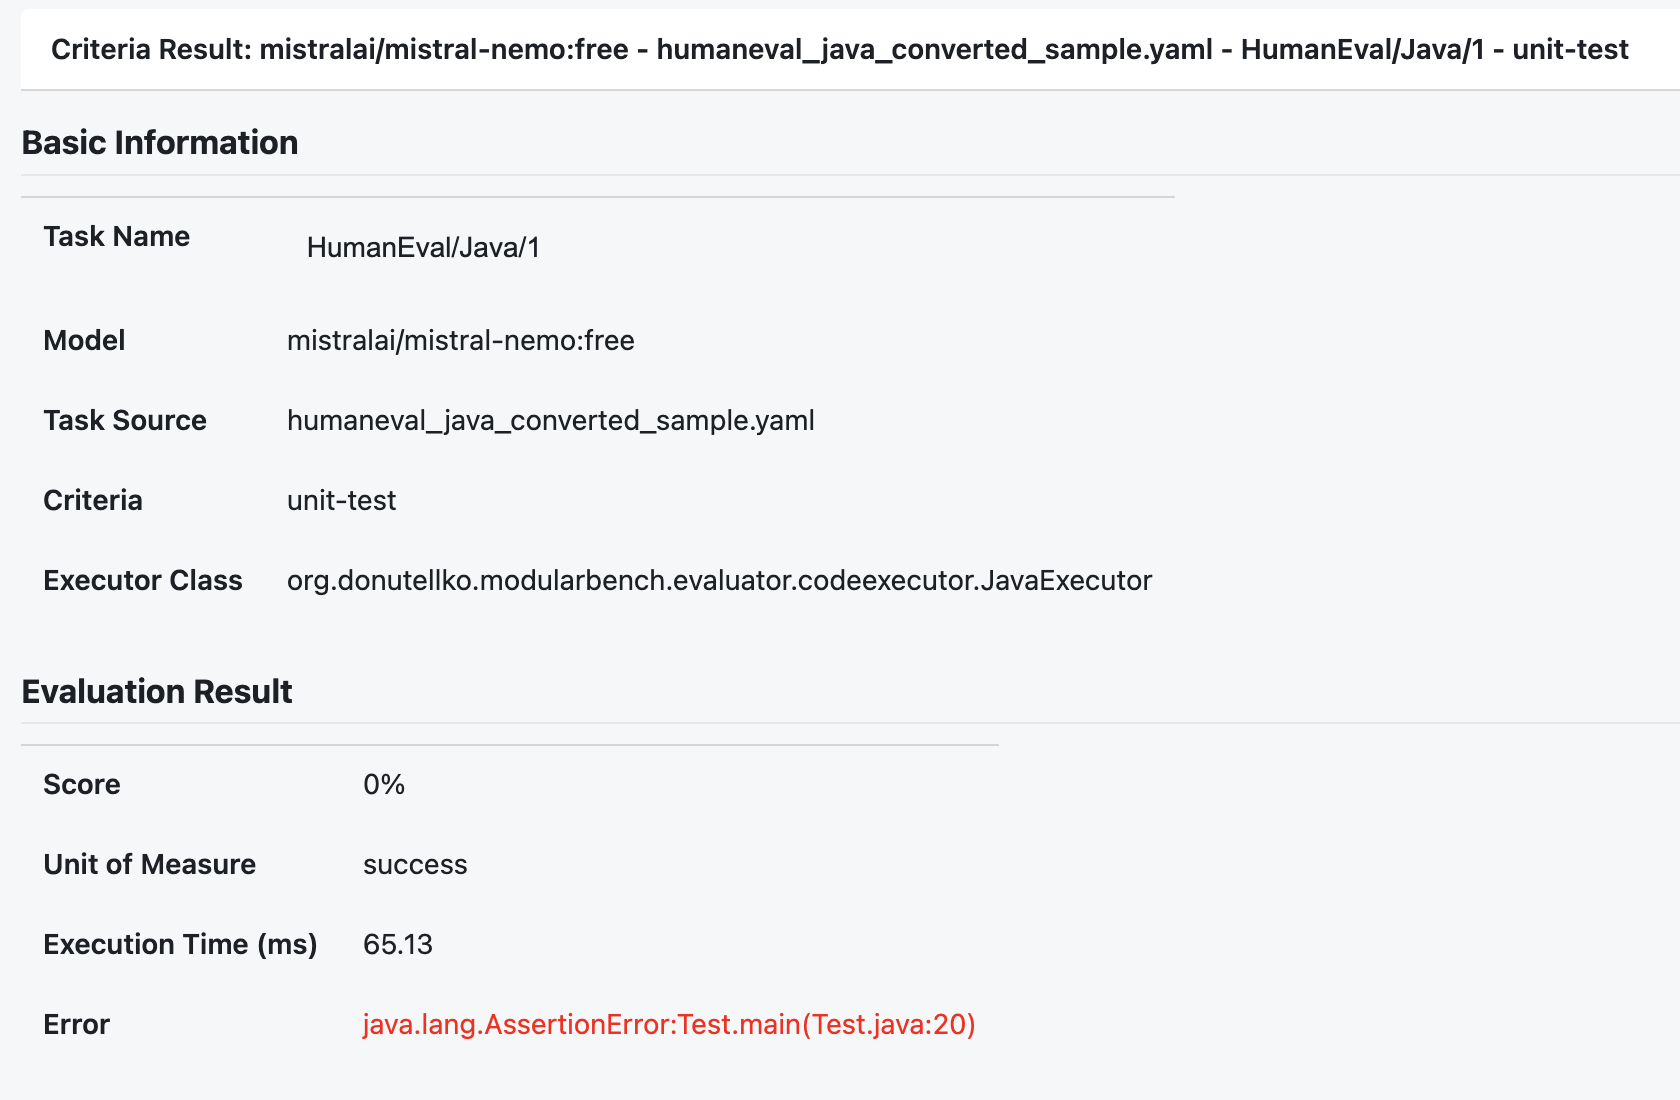
\includegraphics[width=0.9\textwidth]{images/ui_result_test_failure}
    \caption{Example of an error in unit test execution for a specific task and model}
    \label{figure:ui_result_test_failure}
\end{figure}

This level of investigation would not be possible without having the rich output, and would be more difficult without having a UI for browsing them.

Thus, this example demonstrates its effectiveness of the benchmarking framework in providing detailed insights into model performance across multiple dimensions.

\subsection{Comparison with Existing Frameworks}

Table~\ref{tab:framework-comparison-with-proposed} compares the proposed framework with bigcode-evaluation-harness and lm-evaluation-harness.

\begin{landscape}
\begin{longtable}{|p{4cm}|p{5cm}|p{5cm}|p{5cm}|}

% \hline \multicolumn{1}{|c|}{\textbf{Feature}}
% & \multicolumn{1}{c|}{\textbf{bigcode-evaluation-harness}}
% & \multicolumn{1}{c|}{\textbf{lm-evaluation-harness}}
% & \multicolumn{1}{c|}{\textbf{proposed benchmarking framework}} \\
% \hline
% \endhead

       \hline
       \textbf{Feature} & \textbf{bigcode-evaluation-harness} & \textbf{lm-evaluation-harness} & \textbf{proposed benchmarking framework} \\
        \hline
        Specialization & Majorly, code writing tasks, but also allows for documentation generation tasks and natural language reasoning tasks & A universal harness supporting a wide range of tasks & Ecologically concious, taking the most information out of a test and a generated solution \\
        \hline
        Included benchmarks & MBPP, MBPP+, DS-1000, MultiPL-E, Mercury, GSM8K, etc. & MBPP, HumanEval, SpanishBench, basqueGLUE, and many more. & HumanEval for Python and Java, MBPP. \\
        \hline
        Adding tasks, datasets & Requires source code modification & Requires source code modification & With UI or by editing a YAML file editing \\
        \hline
        Available configuration & Task dataset name, Number of tasks, Temperature, Saving LLM responses, Limits of LLM response, etc. & Task datasets list (other parameters are is defined on task level), Limits of LLM response, System prompt, etc. & Task dataset and filters (difficulty, domain, language), Criteria to use (unit-tests, token count, code quality, etc.), Caching generations, test code in prompts \\
        \hline
        Extended output & LLM response or references as JSON & Prompt, LLM response, and metrics results as JSON & Detailed with generations results, metrics, test assertion errors  \\
        \hline
        Run interface & CLI-based, no GUI & CLI-based, no GUI, an API for training loops & Web UI and CLI \\
        \hline
        Result analysis & Overall numeric metric, LLM responses saved in files & Overall numeric metric & Detailed for each metric: with evaluation details and generated solutions  \\
        \hline
        Visualization & No visualization tools & No visualization tools & An UI to edit datasets, configure runs, browse its results \\
        \hline
        Multiple LLMs & One model per run & One model per run & Multiple models per run\\
        \hline
        Load model via transformers & Yes & Yes & No \\
        \hline
        Cache LLM responses & No & Yes with a flag & Yes, in run configuration \\
        \hline

\caption{Comparison of the proposed framework with bigcode-evaluation-harness and lm-evaluation-harness}
\label{tab:framework-comparison-with-proposed}
\end{longtable}
\end{landscape}

As we can see from the table, the proposed framework offers several advantages over existing solutions.
It supports multiple models per run, allowing for direct comparison under identical conditions.
The web interface makes it accessible, and the detailed and visual output facilitates in-depth analysis of results.
Moreover, the configuration is highly flexible, enabling researchers to tailor benchmarks to their specific needs.
Unlike bigcode-evaluation-harness, the framework allows for caching LLM responses, making it more efficient and environmentally friendly for repeated experiments.

As a downside, the proposed framework currently supports a more limited set of tasks and datasets compared to the other two.
And it lacks the support for loading models via the \texttt{transformers} library, which may be a limitation for researchers who want to evaluate local models.

\subsection{Results Discussion and Limitations}

The current prototype demonstrates that the proposed approach is viable and already supports the core functionalities needed to run benchmarks and collect meaningful results.
At the same time, it remains a prototype and lacks several features required for reliable use in real research and production settings.

First, the execution environment is not sufficiently isolated.
Changes in the host machine may affect execution time and distort metrics such as CPU usage.
A more robust sandboxing mechanism is needed to ensure reproducibility.
Moreover, the system currently supports only a subset of programming languages.
Extending test execution to other widely used languages would broaden applicability.
To address these issues, the code and tests should be run in a Docker environment or using a specialized solution.

Second, while the prototype allows shared use on a common server, it raises concerns about data consistency and security.
Proper authorization, as well as locking mechanisms for files being edited, should be implemented to support collaborative scenarios safely.

Third, although the user interface already covers the essential operations, further improvements are necessary to make it more convenient and user-friendly.
Currently, in order to use the prototype, an in-depth understanding of the system is required.

Finally, before results produced by this benchmark can be used in scientific studies, datasets need to be expanded and standardized.
Feedback from experienced researchers and developers will also be critical for validating the approach and guiding its further development.

\section{Conclusion and Future Work}

Benchmarks play a central role in the development of large language models and in guiding their use in real-world applications.
In this work, we analyzed existing benchmarks and harnesses and found that each approach has its own limitations.
Benchmarks become saturated, suffer from data leakage, support only a limited set of metrics or languages, and most consume significant energy and computational resources.
Harnesses, in turn, often lack detailed analysis of results and do not provide convenient mechanisms for comparing models across multiple metrics.
Different benchmarks partially compensate for each other, but none of them is universal.

To address these issues, we proposed an approach that maximizes the insights gained from each benchmark run.
By combining multiple evaluation criteria within a single execution, the framework increases the usefulness of results for researchers and practitioners, while at the same time reducing the environmental impact of benchmarking by limiting redundant runs.
To demonstrate the feasibility of this idea, we implemented a prototype system and validated its basic functionality.
The prototype confirms that it is possible to integrate traditional program analysis metrics with LLM-based evaluations, while also highlighting several challenges that need to be solved before such a tool can be used in practice.

The system integrates a backend with a REST API, a frontend interface, and a configuration mechanism based on declarative YAML files.
The prototype demonstrates that benchmarks can be executed with different combinations of task sources and execution settings, producing results that include both traditional metrics, such as unit tests and static analysis, and LLM-based evaluations.

The experiments with the prototype illustrated the complete pipeline: uploading task sources and configurations, launching benchmarks, monitoring their progress, and inspecting results.
Even with a small number of tasks and languages, the system proved that such a workflow is feasible and can support different benchmarking scenarios.

The current implementation remains a prototype.
It lacks isolated execution environments, which makes performance-related metrics sensitive to the conditions of the host machine.
Test execution is supported only for a subset of programming languages, and collaborative use on a shared server would require authentication and file locking.
Datasets also need to be expanded and standardized before results could be reliably applied in research.

Future work should address these limitations by improving execution isolation, extending language support, and refining the user interface.
Security and collaboration features will be necessary for real-world deployment.
Finally, before the approach can be adopted more widely, it will be important to collect feedback from the research community and adjust the design accordingly.
